% !TeX root = main.tex
\section*{Introduction}
The difference between a positive and a negative mask is investigated. Contact lithography was used.

\section*{Lithographic system}
Optical contact lithography was used.
\begin{figure}[H]
	\centering
	\resizebox{0.7\linewidth}{!}{% !TeX root = main.tex
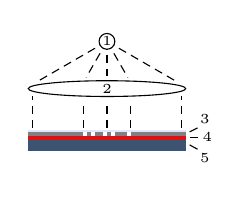
\begin{tikzpicture}
    % Sample
    \fill[fill={rgb:red,66;green,91;blue,121}] (-1,-1.24) rectangle (1,-1.39);
    \draw (1.05,-1.315) to node [below right = -.4 mm] {\tiny $5$} (1.15,-1.37);
    % Resist
    \fill[fill={rgb:red,198;green,15;blue,15}] (-1,-1.20) rectangle (1,-1.24);
    \draw (1.05,-1.22) to node [right = -.1 mm] {\tiny $4$} (1.15,-1.22);
    % Mask
    \foreach \x/\y in {0/.7,.75/.8,.85/0.95,1/1.05,1.1/1.25,1.3/2}
        \fill[fill=gray] (\x-1,-1.15) rectangle (\y-1,-1.20);
    \draw (1.05,-1.15) to node [above right = -.4 mm] {\tiny $3$} (1.15,-1.10);
    % Glass plate
    \fill[fill=blue!10] (-1,-1.12) rectangle (1,-1.15);
    % Lens
    \draw (0,-.6) ellipse [x radius=1, y radius=.1] node {\tiny $2$};
    % Light rays
    \foreach \angle/\r in {210/1,240/.53,270/.44,300/.53,330/1}
        \draw[densely dashed] (0,0) -- (\angle:\r);
    \foreach \x/\y in {-.95/.7,-.3/.75,0/.75,.3/.75,.95/.7}
        \draw[densely dashed] (\x,-1.1) -- (\x,-\y);
    % Light source
    \draw[fill=white] (0,0) ellipse [x radius=.1, y radius=.1] node {\tiny $1$};
\end{tikzpicture}
}
	\caption{Polymer changes}
	\label{fig:contact-litho}
\end{figure}
A mask was created, with both the original design and an inverted version.

\section*{Substrate and resist}
A series of square cut silicon substrates of a by a mm \todo[inline]{approximate dimensions} were used. Resist consists of polymers...

\begin{figure}[H]
	\centering
	\begin{subfigure}[t]{0.45\linewidth}
		\centering
		\resizebox{\linewidth}{!}{% !TeX root = main.tex
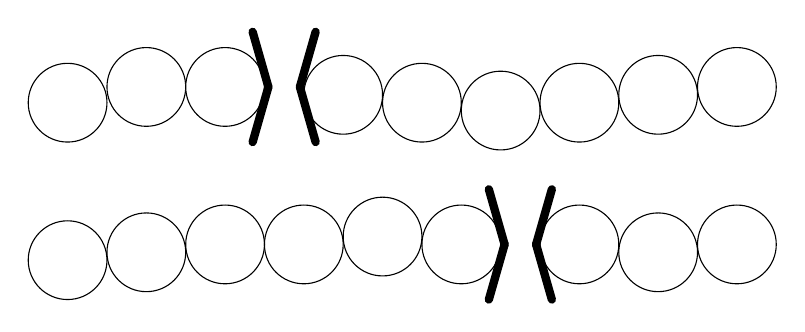
\begin{tikzpicture}
    % Polymer beads
    \foreach \x/\y in {0/0,1/.1,2/.2,3/.2,4/.3,5/.2,6.5/.2,7.5/.1,8.5/.2}
        \draw (\x,\y) circle (5mm);
    % Polymer beads
    \foreach \x/\y in {0/0,1/.2,2/.2,3.5/.1,4.5/0,5.5/-.1,6.5/.0,7.5/.1,8.5/.2}
        \draw[black,fill=white] (\x,2+\y) circle (5mm);
    % Scissors
    \begin{scope}[line width=3,line cap=round]
        % Left scissor
        \draw (5.55,.2) -- (5.35,.9);
        \draw (5.55,.2) -- (5.35,-.5);
        % Right scissor
        \draw (5.95,.2) -- (6.15,.9);
        \draw (5.95,.2) -- (6.15,-.5);
        
        % Left scissor
        \draw (2.55,2.2) -- (2.35,2.9);
        \draw (2.55,2.2) -- (2.35,1.5);
        % Right scissor
        \draw (2.95,2.2) -- (3.15,2.9);
        \draw (2.95,2.2) -- (3.15,1.5);
    \end{scope}
\end{tikzpicture}
}
		\caption{Chain scissors}
		\label{fig:chainscissor}
	\end{subfigure}
	~
	\begin{subfigure}[t]{0.45\linewidth}
		\centering
		\resizebox{\linewidth}{!}{% !TeX root = main.tex
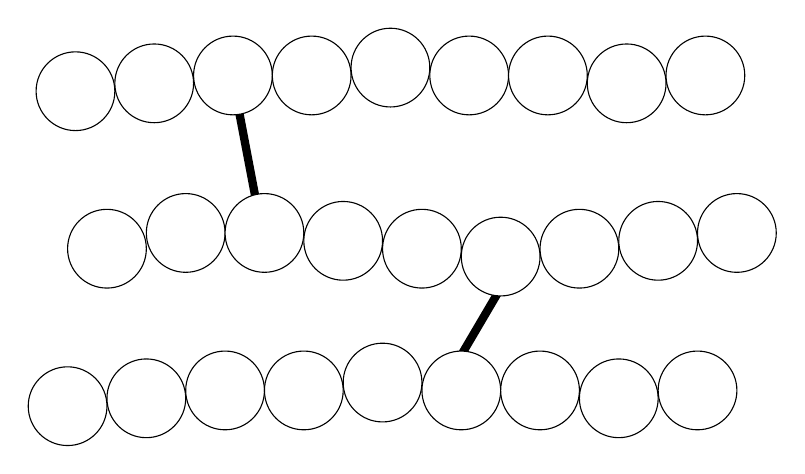
\begin{tikzpicture}
    % Cross links
    \begin{scope}[line width=3]
        \draw (5,.65) -- (5.5,1.5);
        \draw (2.5,2.05) -- (2.1,4.15);
    \end{scope}
    % Polymer beads
    \foreach \x/\y in {0/0,1/.1,2/.2,3/.2,4/.3,5/.2,6/.2,7/.1,8/.2}
        \draw[black,fill=white] (\x,\y) circle (5mm);
    % Polymer beads
    \foreach \x/\y in {0/0,1/.2,2/.2,3/.1,4/0,5/-.1,6/.0,7/.1,8/.2}
        \draw[black,fill=white] (.5+\x,2+\y) circle (5mm);
    % Polymer beads
    \foreach \x/\y in {0/0,1/.1,2/.2,3/.2,4/.3,5/.2,6/.2,7/.1,8/.2}
        \draw[black,fill=white] (.1+\x,4+\y) circle (5mm);
\end{tikzpicture}
}
		\caption{Cross-linking}
		\label{fig:crosslinking}
	\end{subfigure}
	\caption{Polymer changes}
	\label{fig:polymers}
\end{figure}

\todo[inline]{polymer chain images}

\section*{Recipe}
The recipes for both the positive and negative resists are explained here.
\subsection*{Positive resist}
For the positive tone resist the primer \todo[inline]{wat voor primer?} is deposited by hand on top of a silicon wafer and spun for \todo[inline]{wat voor recipe? hoe lang en hoe hard wil je hem hebben?} minutes at ???? RPM. The primer is baked on a hot plate at 200$^{\circ}$~C for two minutes. Then AZ5214 \todo[inline]{dubbelchecken of dit wel de juiste resist is, okay?} is used as the resist layer by depositing it on top of the primer and spinning it with the same recipe as the primer. The resist is baked on a hot plate at 90$^{\circ}$~C for one minute. The sample is then exposed to a close contact/proximity \todo[inline]{welke van de twee is het?} exposure for a variable amount of minutes \todo[inline]{give range of minutes used}, after which it is developed for 60 seconds in \todo[inline]{???} and then development is stopped by rinsing the sample another 60 seconds in purified water.

\subsection*{Negative resist}
For the negative resist samples, the same AZ2512 is used, but with a slightly different recipe to make it negative tone. Up to the exposure, the negative resist recipe is the same as that for the positive tone. 

Using the same mask as for the positive exposure, the sample is illuminated for a period 1 \todo[inline]{check time} minutes. After this first illumination the sample is baked in an oven at ... \todo[inline]{temp?} $^\circ$~C for 45 seconds. During this time cross-links are formed in the resist that was exposed during the first illumination. During baking the sample lies on an aluminium slab inside the oven, this prevents a large decrease in temperature when the oven door is opened and ensures good heat transfer to the sample. After baking, the entire sample is exposed (flood exposure) for a period of either 1,2,3,4 \todo[inline]{all times} minutes. During this time the polymer chains in the areas of the resist that were not exposed during the first illumination, are cut up into smaller chains. In the next step, the development, these smaller chains are dissolved in the development solution \todo[inline]{name}. After development, the sample is rinsed with purified water as was done with the positive resist samples.